\documentclass{article}

\setlength{\headsep}{0.75 in}
\setlength{\parindent}{0 in}
\setlength{\parskip}{0.1 in}

%=====================================================
% Add PACKAGES Here (You typically would not need to):
%=====================================================

\usepackage{xcolor}
\usepackage[margin=1in]{geometry} % Used for page margins, often replaces fullpage
\usepackage{amsmath,amsthm,amssymb} % amssymb added for common math symbols

\usepackage{enumitem} % For custom list environments

\usepackage{tcolorbox}
% \usepackage{fullpage} % Geometry handles this better
\usepackage[parfill]{parskip} % For paragraph spacing
\usepackage{hyperref}
\usepackage[nameinlink, capitalise]{cleveref} % For smart referencing

\usepackage{algorithm2e} % For algorithms
\usepackage{tikz} % For drawing diagrams
\usepackage{siunitx} % For units
\usepackage{graphicx}

\usetikzlibrary{arrows.meta, positioning}

\crefname{algocf}{Algorithm}{Algorithms}

\RestyleAlgo{ruled} % Style for algorithms

\definecolor{linkc}{rgb}{0.1, 0.5, 0.7}
\definecolor{citec}{rgb}{0.6, 0.3, 0.7}
\definecolor{urlc}{rgb}{0.5, 0.1, 0.2}
\hypersetup{
  colorlinks=true,
  linkcolor=linkc,
  citecolor=citec,
  urlcolor=urlc
}

\renewcommand{\d}{\,\mathrm{d}} % Differential d

%=====================================================
% Ignore This Part (But Do NOT Delete It:)
%=====================================================

\theoremstyle{definition}
\newtheorem{problem}{Problem}
\newtheorem*{fun}{Fun with Algorithms}
\newtheorem*{challenge}{Challenge Yourself}
\def\fline{\rule{0.75\linewidth}{0.5pt}}
\newcommand{\finishline}{
  \begin{center}\fline
\end{center}}
\newtheorem*{solution*}{Solution}
\newenvironment{solution}{
\begin{solution*}}{{\finishline}
\end{solution*}}
\newcommand{\grade}[1]{\hfill{\textbf{($\mathbf{#1}$ points)}}}
\newcommand{\thisdate}{\today}
\newcommand{\thissemester}{\textbf{Rutgers: Spring 2026}}
\newcommand{\thiscourse}{CS 344: Algorithms}
\newcommand{\thishomework}{Number}
\newcommand{\thisname}{Name}
\newcommand{\thisextension}{Yes/No}

\headheight 40pt
\headsep 10pt

\newcommand{\thisheading}{
  \noindent
  \begin{center}
    \framebox{
      \vbox{\vspace{2mm}
        \hbox to 6.28in { \textbf{\thiscourse \hfill \thissemester} }
        \vspace{4mm}
        \hbox to 6.28in { {\Large \hfill Homework \#\thishomework \hfill} }
        \vspace{2mm}
        \hbox to 6.28in { { \hfill \hfill} }
        \vspace{2mm}
        \hbox to 6.28in { \emph{Name(s): \thisname \hfill }}
      \vspace{2mm}}
    }
  \end{center}
  \bigskip
}

%=====================================================
% Some useful MACROS (you can define your own in the same exact way also)
%=====================================================

\newcommand{\ceil}[1]{{\left\lceil{#1}\right\rceil}}
\newcommand{\floor}[1]{{\left\lfloor{#1}\right\rfloor}}
\newcommand{\prob}[1]{\Pr\paren{#1}}
\newcommand{\expect}[1]{\Exp\bracket{#1}}
\newcommand{\var}[1]{\textnormal{Var}\bracket{#1}}
\newcommand{\set}[1]{\ensuremath{\left\{ #1 \right\}}}
\newcommand{\poly}{\mbox{\rm poly}}

%=====================================================
% Fill Out This Part With Your Own Information:
%=====================================================

\renewcommand{\thishomework}{2} %Homework number
\renewcommand{\thisname}{Iris$_1$ Martinez$_1$} % Enter your name here

\begin{document}

\thisheading

\subsection*{Homework Policy}
\begin{itemize}
  \item You may consult all course materials (lecture notes, textbook, slides, etc.) while writing your solutions. No external resources are permitted.

  \item \textbf{All submissions should be typeset in LaTeX, handwritten solutions are not accepted}.

  \item Remember to always \textbf{prove the correctness} of your algorithms and \textbf{analyze their running time} (or any other efficiency measure asked in the question).

  \item Homework assignments are completed and submitted in fixed groups of 3 students. Only \textbf{one member of the group submits} the full solution on Canvas. The submission must include the names of all group members. The other two members do \textbf{not need to submit anything separately}.

  \item You may discuss the problems with any of your classmates, even those outside your group. However, \textbf{each group must write and submit their solutions independently}.

  \item Attempt the challenge problems only if you find them interesting.
\end{itemize}

\subsection*{Acknowledgment (to be reviewed and edited as needed)}
\begin{tcolorbox}[colframe=black,colback=white,arc=5mm]
  I, \textbf{Iris Martinez} consulted with (yada yada yada). \textbf{I hereby affirm that all external assistance utilized in the preparation of this document has been properly acknowledged}.
\end{tcolorbox}

\finishline
\newpage

\newpage

%=====================================================
% PROBLEM 1: LOCAL MINIMUM
%=====================================================

\begin{problem}
  You are given an array \( A[1..n] \) with the following properties:
  \begin{itemize}
    \item \( A[1] > A[2] \) (the first element is greater than the second).
    \item \( A[n-1] \leq A[n] \) (the second-to-last element is less than or equal to the last).
  \end{itemize}

  A \textbf{local minimum} is an element \( A[x] \) such that:
  \[
    A[x-1] \geq A[x] \leq A[x+1].
  \]
  For example, in the array \( A = [9, 7, 7, 2, 1, 3, 7, 5, 4, 7, 3, 3, 4, 8, 6, 9, 6] \), there are six local minima.

  Design an \( O(\log n) \)-time algorithm to find a local minimum.

\end{problem}

\begin{solution}

  %=================================================
  % 1. THE ALGORITHM %=====================================================

  %=================================================
  % 2. PROOF OF CORRECTNESS %=====================================================

  %=================================================
  % 3. RUN TIME ANALYSIS %=====================================================

\end{solution}

\newpage

\begin{problem}
  Suppose you are given two sorted arrays $A[1 . . n]$ and $B[1 . . n]$ containing distinct integers. Describe a $O(\log n)$ algorithm to find the median (meaning the $n$th smallest element) of the union $A \cup B$. For example, given the input

  $$
  A[1 . .8]=[0,1,6,9,12,13,18,20] \quad B[1 . .8]=[2,4,5,8,17,19,21,23]
  $$

  your algorithm should return the integer 9. [Hint: What can you learn by comparing one element of $A$ with one element of $B$ ?]

\end{problem}

\begin{solution}

  %=================================================
  % 1. THE ALGORITHM %=====================================================

  %=================================================
  % 2. PROOF OF CORRECTNESS %=====================================================

  %=================================================
  % 3. RUN TIME ANALYSIS %=====================================================

\end{solution}

\newpage

\begin{problem}
  Write an algorithm in pseudocode:

  \begin{itemize}
    \item Input: An array $A$ with $n$ distinct (non-equal) elements
    \item Output-1: numbers $x$ and $y$ in $A$ that minimize $|x-y|$, where $|x-y|$ denotes absolute-value(x-y). (If there are multiple closest pairs, you only have to return one of them.)
    \item Output-2: a pair of numbers $w$ and $z$ in $A$ that minimize $|w+z|.$
  \end{itemize}
  The run-time should be significantly better than $O(n^2)$.

\end{problem}

\begin{solution}

  %=================================================
  % 1. THE ALGORITHM %=====================================================

  %=================================================
  % 2. PROOF OF CORRECTNESS %=====================================================

  %=================================================
  % 3. RUN TIME ANALYSIS %=====================================================

\end{solution}

\newpage

\begin{problem}
  An inversion (swap) in an array $A[1 . . n]$ is a pair of indices $(i, j)$ such that $i<j$ and $A[i]>A[j]$. The number of inversions in an $n$-element array is between 0 (if the array is sorted) and $\binom{n}{2}$ (if the array is sorted backward). Describe and analyze an algorithm to count the number of inversions in an $n$-element array in $O(n \log n)$ time. [Hint: Modify mergesort.]
\end{problem}

\begin{solution}

  %=================================================
  % 1. THE ALGORITHM %=====================================================

  %=================================================
  % 2. PROOF OF CORRECTNESS %=====================================================

  %=================================================
  % 3. RUN TIME ANALYSIS %=====================================================

\end{solution}

\newpage

\begin{problem}
  Given an array \( A \) of length \( n \), and two indices \( i \) and \( j \) with \( i \leq j \), define \( \text{Prod}(A,i,j) \) as the product of elements from \( A[i] \) to \( A[j] \), i.e., \( A[i] \times A[i+1] \times \cdots \times A[j] \). If \( i = j \), then \( \text{Prod}(i,j) = A[i] \).

  For example, if \( A = [3, 0.1, 5, 20, 4] \), then \( \text{Prod}(A,1,3) = 0.1 \times 5 \times 20 = 10 \).

  Now, consider the following problem MaxProd(A):

  \begin{itemize}
    \item \textbf{Input}: An array \( A \) of length \( n \) where all elements are positive, but may include fractional values (e.g., \( A[i] = 0.1 \) is valid).
    \item \textbf{Output}: The maximum possible value of \( \text{Prod}(A, i, j) \) for some subarray \( A[i..j] \).
  \end{itemize}

  For example, if \( A = [3, 0.2, 4, 0.5, 1, 4, 0.3, 2] \), the maximum product is \( 8 \), which is achieved by the subarray \( [4, 0.5, 1, 4] \).

\begin{enumerate}[label=\alph*)]
  \item

    Write pseudocode for a recursive algorithm \( \text{MaxProd}(A) \) that solves the problem in \( O(n\log n) \) time. You only need to provide the pseudocode and the recurrence relation for the algorithm.

    \textit{Hint}: The recurrence formula is similar to one we've used before, so you don't need to prove that it solves to \( T(n) = O(n \log n) \).

    \textit{Note}: While there are faster, non-recursive algorithms for this problem, you must use a recursive algorithm for this homework.

    \begin{solution}

      %=================================================
      % 1. THE ALGORITHM %=====================================================

      %=================================================
      % 2. PROOF OF CORRECTNESS %=====================================================

      %=================================================
      % 3. RUN TIME ANALYSIS %=====================================================

    \end{solution}

  \item Now, write pseudocode for a recursive algorithm that solves the problem in \( O(n) \) time. As in Part 1, provide the pseudocode and the recurrence relation for the algorithm.

    \textit{Hint}: Similar to the Max Profit problem covered in class, solve a helper problem \( \text{MaxProdX}(i, j) \), which gives additional information beyond just the maximum product.

    If you're confident with the \( O(n) \) algorithm, you can directly write a single solution for both Part 1 and Part 2. However, if you're unsure, first implement the \( O(n \log n) \) solution for Part 2, then write the separate \( O(n) \) algorithm.
\end{enumerate}
\end{problem}

\begin{solution}

%=================================================
% 1. THE ALGORITHM %=====================================================

%=================================================
% 2. PROOF OF CORRECTNESS %=====================================================

%=================================================
% 3. RUN TIME ANALYSIS %=====================================================

\end{solution}

\newpage

\begin{problem}
You are given two strings $A$ and $B$ of length $n$, each consisting of possibly repeated characters from an alphabet of size $M$. Two strings $A$ and $B$ are said to be \textbf{anagrams} of one another if it is possible to reorder the characters in $A$ to obtain string $B$ (without removing or adding any characters). For instance, the strings ``ELEVEN PLUS TWO'' and ``TWELVE PLUS ONE'' are anagrams of one another (think of empty-space  also as a character in the alphabet).

\smallskip

Your goal is to design an algorithm that decides if a given pair of strings are anagrams of one another.
You may assume that all characters in the alphabet can represented by distinct integers in the set $\set{1,2,\ldots,M}$, and that you can convert any character to its integer representation in $O(1)$ time (note that $M$ can be much larger than $n$).
\smallskip

\begin{enumerate}
  \item[(a)] Design an algorithm for this problem with worst-case  runtime of $O(n+M)$.

    \begin{solution}

      %=================================================
      % 1. THE ALGORITHM %=====================================================

      %=================================================
      % 2. PROOF OF CORRECTNESS %=====================================================

      %=================================================
      % 3. RUN TIME ANALYSIS %=====================================================

    \end{solution}

  \item[(b)] Design a randomized algorithm for this problem with worst-case expected runtime of $O(n)$.

    \begin{solution}

      %=================================================
      % 1. THE ALGORITHM %=====================================================

      %=================================================
      % 2. PROOF OF CORRECTNESS %=====================================================

      %=================================================
      % 3. RUN TIME ANALYSIS %=====================================================

    \end{solution}

\end{enumerate}

\end{problem}

\newpage

\begin{problem}
Suppose we have an array $A[1:n]$ which consists of numbers $\set{1,\ldots,n}$ written in some arbitrary order (this means that $A$ is a \emph{permutation} of the set $\set{1,\ldots,n}$).
Our goal in this problem is to design a very fast randomized algorithm that can find an index $i$ in this array such that $A[i] \mod 5 = 0$, i.e., $A[i]$ is divisible by five.
For simplicity, in the following, we assume that $n$ itself is a multiple of $5$ and
is at least $5$ (so a correct answer always exist).

For instance, if $n=10$ and the array is $A=[8,7,2,5,4,6,3,1,10,9]$, we can output either of indices $4$ or $9$.

\begin{enumerate}
  \item[(a)]  Suppose we sample an index $i$ from $\set{1,\ldots,n}$ uniformly at random. What is the probability that $i$ is a correct answer, i.e., $A[i] \mod 5 = 0$?

    \begin{solution}

    \end{solution}

  \item[(b)] Suppose we sample $m$ indices from $\set{1,\ldots,n}$ uniformly at random and with repetition. What is the probability that none of these indices is a correct answer?  \grade{5}
\end{enumerate}

\begin{solution}

\end{solution}

Now, consider the following simple algorithm for this problem:

\textbf{Find-Index-1$(A[1:n])$:}
\begin{itemize}
  \item Let $i=1$.  While $A[i] \mod 5 \neq 0$, sample $i \in \set{1,\ldots,n}$ uniformly at random. Output $i$.
\end{itemize}

The proof of correctness of this algorithm is straightforward and we skip it in this question.

\begin{enumerate}
  \item[(c)] What is the worst-case \textbf{expected} running time of \textbf{Find-Index-1$(A[1:n])$}? Remember to prove your answer formally.
\end{enumerate}

The problem with \textbf{Find-Index-1} is that in the worst-case (and not in expectation), it may actually never terminate! For this reason, let us consider
a simple modification to  this algorithm as follows.

\textbf{Find-Index-2$(A[1:n])$:}
\begin{itemize}
  \item For $j=1$ to $n$:
    \begin{itemize}
      \item Sample $i \in \set{1,\ldots,n}$ uniformly at random and if $A[i] \mod 5 = 0$, output $i$ and terminate; otherwise, continue.
    \end{itemize}
  \item If the for-loop never terminated, go over the array $A$ one element at a time to find an index $i$ with $A[i] \mod 5 =0$ and output it as the answer.
\end{itemize}

\begin{solution}

\end{solution}

Again, we skip the proof of correctness of this algorithm.

\begin{enumerate}
  \item[(d)] What is the \textbf{worst-case running time} of \textbf{Find-Index-2$(A[1:n])$}? What about its worst-case \textbf{expected} running time? Remember to prove your answer formally.

\end{enumerate}

\end{problem}

\begin{solution}

\end{solution}

\newpage

\finishline

\begin{challenge}
Following are some variation of the Tower of Hanoi problem (If you find the solution come and talk to the instructor!):

\begin{enumerate}

  \item If all moves must be between adjacent pegs, what is the number of movies required? That is you cannot directive move from $1$ to $3$ for instance.

  \item

    Now, consider a variation where for each disk size \( k \), there are two identical disks. The goal remains to move all disks from peg \( 1\) to peg \( 3 \) while following the standard Tower of Hanoi rules.
    \begin{center}
      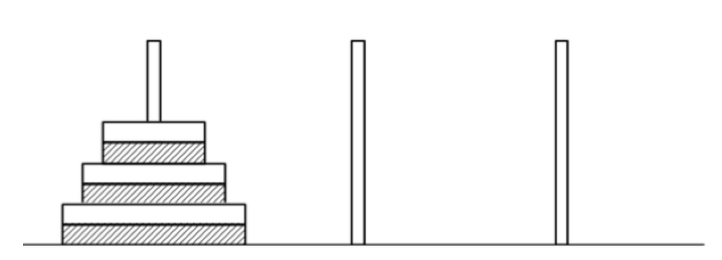
\includegraphics[scale=0.2]{images/hanoi_double.png}
    \end{center}
    \begin{itemize}
      \item If we ignore the fact that disks of the same size are identical and treat them as distinct disks, we can simply apply the standard Tower of Hanoi solution to \( 2n \) disks. What is the recurrence relation and the resulting number of moves?

      \item If we move both disks of the same size simultaneously while using standard Hanoi's algorithm, we are close to the solution. This strategy may flip the order of some equal size disks. Repeat this again to restore the order of disks. How many moves does this take?

      \item   What is the optimal strategy to minimize the number of moves while preserving the original order of the disks?
    \end{itemize}

\end{enumerate}

\end{challenge}

\newpage

\end{document}